\documentclass{standalone}

\usepackage{tikz}
\usepackage{pgf-umlcd}
\usepackage[bitstream-charter]{mathdesign} % +1! taules mes petites i hi caben
\usepackage[T1]{fontenc}
\usepackage[utf8]{inputenc}

\begin{document}

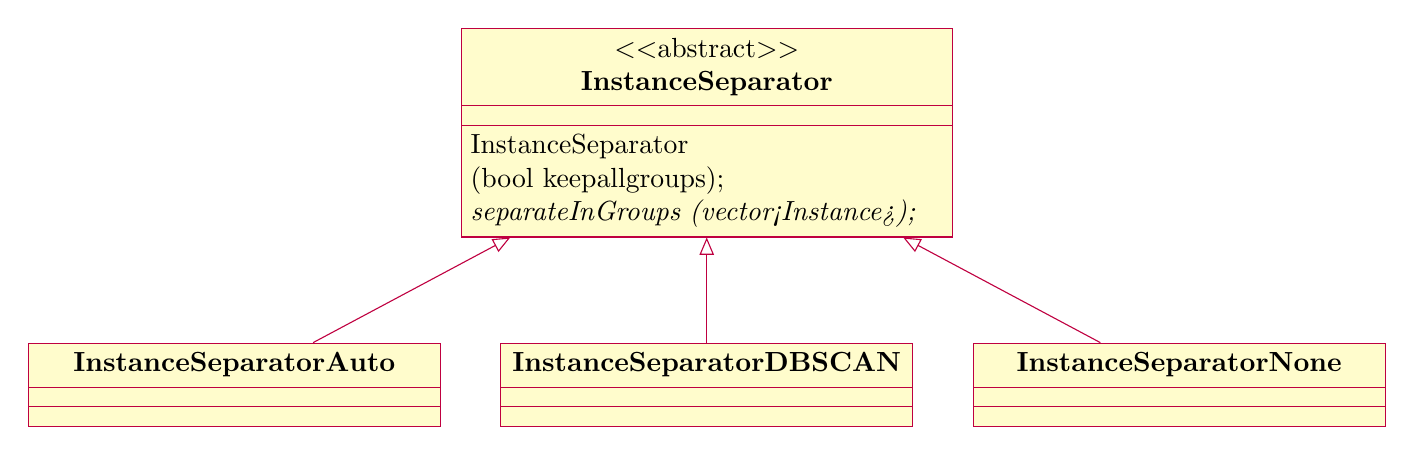
\begin{tikzpicture}

\begin{abstractclass}[text width=6cm]{InstanceSeparator}{0,0}
\operation{InstanceSeparator (bool keepallgroups);}
\operation[0]{separateInGroups (vector<Instance>);}
\end{abstractclass}

\begin{class}[text width=5cm]{InstanceSeparatorAuto}{-6,-4}
\inherit{InstanceSeparator}
\end{class}
\begin{class}[text width=5cm]{InstanceSeparatorDBSCAN}{0,-4}
\inherit{InstanceSeparator}
\end{class}
\begin{class}[text width=5cm]{InstanceSeparatorNone}{6,-4}
\inherit{InstanceSeparator}
\end{class}
\end{tikzpicture}

\end{document}
